% ============================================
% ====== Frame : Plan ========================
% ============================================
{
  \AtBeginSection[]{}
}


% ============================================
% ====== Frame : Continuous model    =========
% ============================================

\section{Forward Discretization}
\subsection{The continuous model}
\begin{frame}{Continuous Forward Model}
  \small
  First order acoustic wave equation:
  \vspace{-0.7cm}
  \begin{multicols}{2}
  \begin{empheq}[left=\empheqlbrace]{align}
    & \frac{1}{\density \velocity^2}\frac{\partial \contP}{\partial t}+\nabla \cdot \contV=f_p \text{~~ on $\boldsymbol{\Omega}$}\\
    & \density\frac{\partial \contV}{\partial t}+\nabla\contP=0  \text{~~ on $\boldsymbol{\Omega}$}\\
    & \contP=0 \text{~~ on $\textcolor{\myred}{\boldsymbol{\Gamma_1}}$} \\
    & \contP - \velocity \density \contV \cdot \normal=0 \text{~~ on $\textcolor{\myblue}{\boldsymbol{\Gamma_2}}$} \\
    & \contP(0) = 0 \text{, ~~~} \contV(0) = 0
  \end{empheq}

  \columnbreak

~ \\
\begin{center}
\renewcommand\tikzscale{1.0}
\begin{figure}[H]
\centering
\includegraphics[scale=2.5]{image/truncated_domain.pdf}
\caption*{Truncated infinite domain.} \label{truncated_domain}
\end{figure}
  \end{center}
  \end{multicols}

\vspace{-0.5cm}
\begin{block}{Quantities of interest:}

\begin{multicols}{2}

\begin{itemize}
\item $\contP$: the pressure (kg.m$^{-1}$.s$^{-2}$)
\item $\contV$: the wavespeed  (m.s$^{-1}$)
\end{itemize}

\columnbreak

\begin{itemize}
\item $\velocity$: velocity  (m.s$^{-1}$)
\item $\density$:  density  (kg.m$^{-3}$)
\item $\bm$:       bulk modulus ($\bm = \density  \velocity^2$) (kg.m$^{-1}$.s$^{-2}$)
\end{itemize}

\end{multicols}
\end{block}

\end{frame}

% ===================================================
% ====== Frame : Discontinuous Galerkin method ======
% ===================================================
\subsection{Discontinuous Galerkin method}
\begin{frame}{Discontinuous Galerkin method}
\vspace{-1.5cm}
Spatial discretization based on Discontinuous Galerkin methods:
\vspace{0.5cm}
\begin{itemize}
\item<1-> Approximation made with discontinuous basis functions
\item<2-> Block diagonal mass matrix
\item<3-> High scalability of the solver \footcite{shraggeSolving3DAcoustic2014} (suitable for HPC environnement)
\item<4-> Deals with unstructured grid (triangles / tetrahedra)
\item<5-> Natural $hp$-adaptivity
\end{itemize}

\begin{overprint}
\onslide<5>
 \begin{multicols}{2}
   \begin{figure}[H]
     \centering
     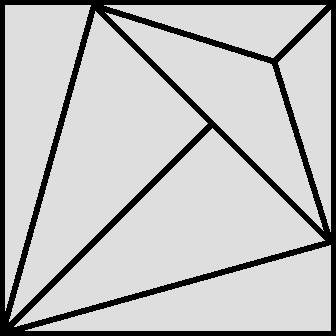
\includegraphics[scale=0.3]{image/h_adaptivity.pdf}
     \caption*{Illustration of \\ $h$-adaptivity.}
     \label{p_adapt_sketch}
   \end{figure}
   \columnbreak
   \begin{figure}[H]
     \centering
     \includegraphics[scale=0.3]{image/p_adaptivity.pdf}
     \caption*{Illustration of \\ $p$-adaptivity.}
     \label{h_adapt_sketch}
   \end{figure}
 \end{multicols}

\onslide<2-4>

\scriptsize
  \begin{empheq}[left=\empheqlbrace]{align}
  & \frac{1}{\bm} \Mass^\element  \frac{\partial \textcolor{\myred}{\coefPolP}^\element}{\partial t}
  + \sum_{d=1}^\dim \Stiff_\xd^\element \textcolor{\myred}{\coefPolVd}^\element
  + \sum_{\Edge} \Mass_\Edge^\element \FluxP^\Edge(\textcolor{\myred}{\coefPolP},\textcolor{\myred}{\coefPolV})
  = \frac{1}{\bm} \Mass^\element \coefpolSource^\element, \\
  & \density \Mass^\element  \frac{\partial \textcolor{\myred}{\coefPolV_d}^\element}{\partial t}
  + \Stiff_\xd^\element \textcolor{\myred}{\coefPolP}^\element + \sum_\Edge \Mass_\Edge \FluxV_d^\Edge (\textcolor{\myred}{\coefPolP},\textcolor{\myred}{\coefPolV})
  = 0  \qquad\text{(for $d=1\,\,\text{to}\,\,\dim$)} \,.
  \label{local_semi_disc2}
  \end{empheq}
\end{overprint}
\vspace{-5cm}

\end{frame}

% ===================================================
% ====== Frame : Speed up studies ===================
% ===================================================

\setbeamercovered{invisible}
\begin{frame}{Scalability Study}{Comparison DG / FD}
\small
Speed up comparison on a 5s simulation in 3D (9km $\times$ 5km $\times$ 3km):

\setlength{\plotwidth}{7cm}
\setlength{\plotheight}{3.7cm}
\begin{figure}[!htbp]
\centering
    \begin{tikzpicture}
      \begin{axis}[%
          width=\plotwidth, height=\plotheight,,
          at={(0,0)},scale only axis,separate axis lines,
          xlabel={\scriptsize{Number of CPU}},
          ylabel={\scriptsize{Speed-up}},
          xmin=1,xmax=768,
%          ymin=0,ymax=1,
          legend pos= north west
          %ymin=0.98,ymax=1.22
        ]
        \addplot[color=black,mark options={solid}, mark=triangle*,
        line width=1.5pt,
        mark size=0pt]
        table[x=monx,y=mony]
        {graph/ideal_speed_up.txt};
        \addlegendentry{\scriptsize{Ideal Speed-up}}
        \addplot[color=blue!80!black,mark options={solid}, mark=triangle*,smooth,
        line width=1pt,
        mark size=0pt]
        table[x=monx,y=mony]
        {graph/dg_speed_up_pres.txt};
        \addlegendentry{\scriptsize{DG}}
        \addplot[color=red,mark options={solid}, mark=*,
        line width=0.8pt,
        mark size=0pt]
        table[x=monx,y=mony]
        {graph/df_speed_up_pres.txt};
        \addlegendentry{\scriptsize{FD}}
\end{axis}
\end{tikzpicture}
\end{figure}

\vspace{-0.2cm}
\uncover<2->{
\begin{block}{\danger Warning}
\small This is an example to illustrate the DG HPC properties. \\
Further comparisons are required to properly compare the two methods.
\end{block}
}

\end{frame}




% ===================================================
% ====== Frame : Time domain motivation =============
% ===================================================
\subsection{Time-Domain}
\begin{frame}{Time-Domain Motivations}

\begin{itemize}
\item<2-> Frequency domain direct-solvers require very large-scale linear systems to solve \footcite{operto20073d}.
\item<3-> Explicit time-schemes do not require the inversion of large size matrices.
\item<4-> In time domain, intermediate results can be stored on the disk to reduce the memory burden (for gradient computation).
\item<5-> In case of disk storage limitation, checkpointing\footcite{griewankAchievingLogarithmicGrowth1992} strategies exists to reduce the overall storage cost.
\end{itemize}

\end{frame}


% ===================================================
% ====== Frame : Time schemes =======================
% ===================================================

\begin{frame}{Time-schemes}
\scriptsize
Three explicit time-schemes as been studied: \\
\begin{multicols}{3}
\textbf{Runge-Kutta 2}

\columnbreak

\textbf{Runge-Kutta 4}

\columnbreak

\textbf{Adams Bashforth 3}
\end{multicols}

\begin{block}{CFL condition\footnotemark}
Initially, the time step $\deltat$ was not computed in the solver.

\begin{multicols}{2}
\begin{equation}
\deltat = \underset{\elementK}{\min}(\deltat^\elementK)\,,
\end{equation}
\begin{equation}
        \deltat^\elementK \le C \frac{r^\elementK}{\velocity^\elementK p^\elementK}\,.
\end{equation}
\vfill

\columnbreak
\tiny
Where:
\begin{itemize}
\item $C$: the CFL condition;
\item $r^\elementK$: the inner radius of the cell $\elementK$;
\item $\velocity^\elementK$: the wavespeed parameter associated to $\elementK$;
\item $p^\elementK$: the polynomial order of approximation in $\elementK$.
\end{itemize}
\end{multicols}
\end{block}
\footcitetext{hesthavenNodalDiscontinuousGalerkin2007}
\end{frame}


\begin{frame}[noframenumbering]{Time-schemes}
\scriptsize
Three explicit time-schemes as been studied: \\
\begin{multicols}{3}
\textbf{Runge-Kutta 2}

\columnbreak

\textbf{Runge-Kutta 4}

\columnbreak

\textbf{Adams Bashforth 3}
\end{multicols}

\begin{block}{CFL condition}
Initially, the time step $\deltat$ was not computed in the solver.

\begin{multicols}{2}
\begin{equation}
\deltat = \underset{\elementK}{\min}(\deltat^\elementK)\,,
\end{equation}
\begin{equation}
        \deltat^\elementK \le C \frac{r^\elementK}{\velocity^\elementK p^\elementK}\,.
\end{equation}
\vfill

\columnbreak
\tiny
Where:
\begin{itemize}
\item $C$: the CFL condition;
\item $r^\elementK$: the inner radius of the cell $\elementK$;
\item $\velocity^\elementK$: the wavespeed parameter associated to $\elementK$;
\item $p^\elementK$: the polynomial order of approximation in $\elementK$.
\end{itemize}
\end{multicols}
\end{block}
\begin{overprint}
\onslide<1>
\begin{figure}[H]
\centering
\includegraphics[scale=0.2]{image/cfl.pdf}
\label{cfl_sketch}
\end{figure}
\onslide<2>
\begin{table}[H]
\centering
\begin{tabular}{|l|l|l|l|}
\hline
  & RK2  & RK4  & AB3  \\ \hline
C & 0.66 & 0.84 & 0.18 \\ \hline
\end{tabular}
\caption*{CFL coefficients for different time schemes.}
\label{coef_cfl}
\end{table}
\end{overprint}

\end{frame}


% ============================================
% ====== Frame : Bernstein Bezier    =========
% ============================================

\subsection{Bernstein-Bézier}
 \begin{frame}{Polynomial bases}
 \scriptsize
 Two polynomial bases has been studied:
 \begin{multicols}{2}
 \textbf{Lagrange} (Nodal)

\vspace{0.5cm}
\begin{figure}[H]
\centering
\setlength{\plotwidth}{3.5cm}
\setlength{\plotheight}{2.5cm}
    \begin{tikzpicture}
      \begin{axis}[%
          width=\plotwidth, height=\plotheight,,
          at={(0,0)},scale only axis,separate axis lines,
          xlabel={$x$},
          %%   ymode=log,
          %yminorticks=true,
           xmin=0,xmax=1,
           %ymin=0,ymax=1,
          legend pos=outer north east
          %ymin=0.98,ymax=1.22
        ]

        %% load current data
        %% -----------------
        \addplot[color=blue!50!black,mark options={solid}, mark=triangle*,
          line width=2pt,
          mark size=0pt]
        table[x=x,y=1]
        {graph/lagrange_5.dat};
        \addlegendentry{$\ell_1^5$}

 \addplot[color=red!75!black,mark options={solid}, mark=*,
          line width=2pt,
          mark size=0pt]
        table[x=x,y=2]
        {graph/lagrange_5.dat};
        \addlegendentry{$\ell_2^5$}

 \addplot[color=green!50!black,mark options={solid}, mark=square*,
          line width=2pt,
          mark size=0pt]
        table[x=x,y=3]
        {graph/lagrange_5.dat};
        \addlegendentry{$\ell_3^5$}

 \addplot[color=yellow!80!black,mark options={solid}, mark=square*,
          line width=2pt,
          mark size=0pt]
        table[x=x,y=4]
        {graph/lagrange_5.dat};
        \addlegendentry{$\ell_4^5$}

 \addplot[color=green!75!white,mark options={solid}, mark=square*,
          line width=2pt,
          mark size=0pt]
        table[x=x,y=5]
        {graph/lagrange_5.dat};
        \addlegendentry{$\ell_5^5$}

 \addplot[color=blue!40!white,mark options={solid}, mark=diamond*,
          line width=2pt,
          mark size=0pt]
        table[x=x,y=6]
        {graph/lagrange_5.dat};
        \addlegendentry{$\ell_6^5$}
      \end{axis}
      %% --------------------------------------------------------------------
    \end{tikzpicture}

\caption*{\scriptsize{Illustration of $P^5([0,1])$ Lagrange basis.}}
\label{lagrange_5}
\end{figure}

\columnbreak
\textbf{Bernstein-Bézier \footcite{chanGPUacceleratedBernsteinBezierDiscontinuous2016}} (Modal)

\begin{figure}[H]
\centering
\setlength{\plotwidth}{3.5cm}
\setlength{\plotheight}{2.5cm}
    \begin{tikzpicture}
      \begin{axis}[%
          width=\plotwidth, height=\plotheight,,
          at={(0,0)},scale only axis,separate axis lines,
          xlabel={$\xx$},
          %%   ymode=log,
          %yminorticks=true,
           xmin=0,xmax=1,
           ymin=0,ymax=1,
          legend pos=outer north east
          %ymin=0.98,ymax=1.22
        ]

        %% load current data
        %% -----------------
        \addplot[color=blue!50!black,mark options={solid}, mark=triangle*,
          line width=2pt,
          mark size=0pt]
        table[x=x,y=50]
        {graph/bb_5.dat};
        \addlegendentry{$B^5_{5,0}$}

 \addplot[color=red!75!black,mark options={solid}, mark=*,
          line width=2pt,
          mark size=0pt]
        table[x=x,y=41]
        {graph/bb_5.dat};
        \addlegendentry{$B^5_{4,1}$}

 \addplot[color=green!50!black,mark options={solid}, mark=square*,
          line width=2pt,
          mark size=0pt]
        table[x=x,y=32]
        {graph/bb_5.dat};
        \addlegendentry{$B^5_{3,2}$}

 \addplot[color=yellow!80!black,mark options={solid}, mark=square*,
          line width=2pt,
          mark size=0pt]
        table[x=x,y=23]
        {graph/bb_5.dat};
        \addlegendentry{$B^5_{2,3}$}

 \addplot[color=green!75!white,mark options={solid}, mark=square*,
          line width=2pt,
          mark size=0pt]
        table[x=x,y=14]
        {graph/bb_5.dat};
        \addlegendentry{$B^5_{1,4}$}

 \addplot[color=blue!40!white,mark options={solid}, mark=diamond*,
          line width=2pt,
          mark size=0pt]
        table[x=x,y=05]
        {graph/bb_5.dat};
        \addlegendentry{$B^5_{0,5}$}
      \end{axis}
      %% --------------------------------------------------------------------
    \end{tikzpicture}

\caption*{\scriptsize{Illustration of $P^5([0,1])$ Bernstein-Bézier basis.}}
\label{bb_base_5}
\end{figure}

\end{multicols}

\uncover<2->{
  \begin{tikzpicture}[remember picture,overlay]
    \draw [red,ultra thick,rounded corners] (0,0) rectangle (6.2,6.5);
  \end{tikzpicture}
}
\end{frame}



% ============================================
% ====== Frame : 1D BB    ====================
% ============================================

\begin{frame}{1D Results using Bernstein-Bézier polynomial basis:}

\begin{figure}[htbp]
\begin{subfigure}{0.45\textwidth}
\centering
\includegraphics[scale=0.2]{image/dx_lag_4.png}
\caption*{$\Diffx$ for Lagrange and $\PolOrder=4$.}
\end{subfigure}
\begin{subfigure}{0.45\textwidth}
\centering
\includegraphics[scale=0.2]{image/dx_bb_4.png}
\caption*{$\Diffx$ for Bernstein and $\PolOrder=4$.}
\end{subfigure}
\begin{subfigure}{0.45\textwidth}
\centering
\includegraphics[scale=0.2]{image/dx_lag_10.png}
\caption*{$\Diffx$ for Lagrange and $\PolOrder=10$.}
\end{subfigure}
\begin{subfigure}{0.45\textwidth}
\centering
\includegraphics[scale=0.2]{image/dx_bb_10.png}
\caption*{$\Diffx$ for Bernstein and $\PolOrder=10$.}
\end{subfigure}
\caption*{Sparsity comparison between Lagrange and Bernstein
$\Diffx$ operator ($\Diffx =  \MassRef^{-1} \StiffRef_\refxx$).}
\label{dx_sparse_pattern}
\end{figure}
\end{frame}

\begin{frame}[noframenumbering]{1D Results using Bernstein-Bézier polynomial basis:}
\setlength{\plotwidth}{6.0cm}
\setlength{\plotheight}{4.5cm}
\begin{figure}[htbp]
\centering
  %% \begin{subfigure}[b]{0.5\textwidth}
    \begin{tikzpicture}
      \begin{axis}[%
          width=\plotwidth, height=\plotheight,,
          at={(0,0)},scale only axis,separate axis lines,xminorticks=true,
          xlabel={Polynomial order $\PolOrder$},
          ylabel={NZV},
          xmin=0,xmax=21,
          legend pos=north west
        ]
        %% load current data
        %% -----------------
        \addplot[color=blue!50!black,mark options={solid}, mark = triangle,
          line width=1pt,
          mark size=2pt]
        table[x=order,y=nzv]
        {graph/Bernstein_sparse.txt};
        \addlegendentry{Bernstein-Bézier}
        \addplot[color=red!50!black,mark options={solid}, mark = *,
          line width=1pt,
          mark size=2pt]
        table[x=order,y=nzv]
        {graph/Lagrange_sparse.txt};
        \addlegendentry{Lagrange}
        %\includegraphics{images/data_bis.pdf}
      \end{axis}
      %% --------------------------------------------------------------------
    \end{tikzpicture}
  %%   \caption{}
  %%   \label{nzv_order}
  %% \end{subfigure}
  %% \begin{subfigure}[b]{0.5\textwidth}
  %%   \setlength{\plotwidth}{6.0cm}
  %%   \setlength{\plotheight}{4.5cm}
  %%   \begin{tikzpicture}
  %%     \begin{axis}[%
  %%         width=\plotwidth, height=\plotheight,,
  %%         at={(0,0)},scale only axis,separate axis lines,xminorticks=true,
  %%         xlabel={Polynomial order $\PolOrder$},
  %%         ylabel={Ratio},
  %%         %%   ymode=log,
  %%         %yminorticks=true,
  %%         xmin=0,xmax=21,
  %%         legend pos=north east
  %%         %ymin=0.98,ymax=1.22
  %%       ]

  %%       %% load current data
  %%       %% -----------------
  %%       \addplot[color=blue!50!black,mark options={solid}, mark = triangle,
  %%         line width=1pt,
  %%         mark size=2pt]
  %%       table[x=order,y=ratio]
  %%       {graph/Bernstein_sparse.txt};
  %%       \addlegendentry{Bernstein-Bézier}
  %%       \addplot[color=red!50!black,mark options={solid}, mark = *,
  %%         line width=1pt,
  %%         mark size=2pt]
  %%       table[x=order,y=ratio]
  %%       {graph/Lagrange_sparse.txt};
  %%       \addlegendentry{Lagrange}
  %%       %\includegraphics{images/data_bis.pdf}
  %%     \end{axis}
  %%     %% --------------------------------------------------------------------
  %%   \end{tikzpicture}
  %%   \caption{}
  %%   \label{ratio_order}
  %% \end{subfigure}

  \caption*{Non zero values (NZV) of the global volume operator as a function of the polynomial order.}
  \label{bb_lag_comp_1d}
\end{figure}

\end{frame}



\begin{frame}[noframenumbering]{2D and 3D Results using Bernstein-Bézier polynomial basis:}
\scriptsize
\vspace{0.5cm}
\begin{table}[H]
    \centering
    \begin{tabular}{|l|l|l|l|l|l|}
    \hline
        \textbf{Sigsbee (2D)} & P1 & P2 & P3 & P4 & P5 \\ \hline
        Number of elements ($\nbelem$) & 569522 & 243636 & 121235 & 66644 & 35929 \\ \hline
        Nodal CPU time (s) & 20628 & 15938 & 14518 & 14649 & 13471 \\ \hline
        Bernstein Bézier CPU time (s) & 41976 & 27660 & 19944 & 15492 & 10960 \\ \hline
        Ratio total CPU time (BB/Nodal) & \cellcolor{\myred!30}2.0 & \cellcolor{\myred!30}1.7 & \cellcolor{\myred!30}1.4 & \cellcolor{\myred!30}1.1 & \cellcolor{\mygreen!30}0.8 \\ \hline
    \end{tabular}
    \caption*{Global CPU time from nodal and Bernstein simulations on the Sigsbee model.}
    \label{sigsbee_bb_tab}
\end{table}

\uncover<2->{
\begin{table}[H]
    \centering
    \begin{tabular}{|l|l|l|l|l|l|}
    \hline
        \textbf{Seam Foothills (reduced) (3D)} & P1 & P2 & P3 & P4 & P5 \\ \hline
        Number of elements ($\nbelem$)          & 401424 & 122806 & 45932 & 20378 & 11299  \\ \hline
        Nodal CPU time (s)          & 42280  & 43080  & 46920 & 54120  & 69960 \\ \hline
        Bernstein CPU time (s)      & 100080 & 62640  & 43560 & 34200 & 33600   \\ \hline
        Ratio total CPU time (BB/Nodal)     & \cellcolor{\myred!30}2.2 & \cellcolor{\myred!30}1.5 & \cellcolor{\mygreen!30}0.9 & \cellcolor{\mygreen!30}0.6 & \cellcolor{\mygreen!30}0.5 \\ \hline
    \end{tabular}
    \caption*{Global CPU time from nodal and Bernstein simulations
    on the reduced Seam foothills model.}
    \label{seam_bb_tab}
\end{table}
}

\end{frame}


% ============================================
% ====== Frame : WADG     ====================
% ============================================

\subsection{Weight Adjusted Discontinuous Galerkin}

\begin{frame}{Weight Adjusted Discontinuous Galerkin (WADG)}
\scriptsize


\uncover<2->{
  \begin{empheq}[left=\empheqlbrace]{align}
  & \frac{1}{\bm} \Mass^\element  \frac{\partial \textcolor{\myred}{\coefPolP}^\element}{\partial t}
  + \sum_{d=1}^\dim \Stiff_\xd^\element \textcolor{\myred}{\coefPolVd}^\element
  + \sum_{\Edge} \Mass_\Edge^\element \FluxP^\Edge(\textcolor{\myred}{\coefPolP},\textcolor{\myred}{\coefPolV})
  = \frac{1}{\bm} \Mass^\element \coefpolSource^\element, \\
  & \density \Mass^\element  \frac{\partial \textcolor{\myred}{\coefPolV_d}^\element}{\partial t}
  + \Stiff_\xd^\element \textcolor{\myred}{\coefPolP}^\element + \sum_\Edge \Mass_\Edge \FluxV_d^\Edge (\textcolor{\myred}{\coefPolP},\textcolor{\myred}{\coefPolV})
  = 0  \qquad\text{(for $d=1\,\,\text{to}\,\,\dim$)} \,,
  \label{local_semi_disc2}
  \end{empheq}
}

  \uncover<3->{
  [Glinsky and Mercerat]\footcite{merceratNodalHighorderDiscontinuous2015}:
  \begin{equation}
[\Mass^\element_\param]_{i,j} = \int_\element \param(\x) \varphi_i^\element(\x) \varphi_j^\element(\x) d\x. \label{local_mass_mercerat}
  \end{equation}
  }


  \uncover<4->{
[Chan et al.] \footcite{chanWeightadjustedDiscontinuousGalerkin2017}:
  \begin{equation}
(\Mass^\element_\param)^{-1} \approx (\Mwadg^\element_\param)^{-1} = (\Mass^\element)^{-1} \Mass^\element_{1/\param} (\Mass^\element)^{-1}.
\label{inv_wadg}
\end{equation}
}


\end{frame}


% ============================================
% ====== Frame : WADG Quadrature point =======
% ============================================

\begin{frame}{Weight Adjusted Discontinuous Galerkin (WADG)}
  \scriptsize
  For sake of accuracy: $\QuadOrder=2\PolOrder+1$.

\begin{table}[]
\begin{tabular}{|l|l|l|l|l|l|l|}
\hline
Polynomial Order ($\PolOrder$)            & 1 & 2  & 3  & 4  & 5  & 6  \\ \hline
Quadrature Order ($\QuadOrder$)           & 3 & 5  & 7  & 9  & 11 & 13 \\ \hline
Number of quadrature points ($n_q$) in 2D & 6 & 7  & 15 & 19 & 28 & 40 \\ \hline
Number of quadrature points ($n_q$) in 3D & 6 & 14 & 31 & 57 & 95 & 146  \\ \hline
\end{tabular}
\caption*{\scriptsize{Number of quadrature points as a function of $\QuadOrder$.}}
\end{table}


  \begin{figure}[!htbp]
    \begin{subfigure}{0.45\textwidth}
      \centering
      \includegraphics[scale=0.07]{image/quad_2d.pdf}
    \end{subfigure}
    \begin{subfigure}{0.45\textwidth}
      \centering
      \includegraphics[scale=0.08]{image/quad_3d.pdf}
    \end{subfigure}
    \caption*{\scriptsize{Quadrature points on 2D and 3D reference element for $\QuadOrder=6$.}}
    \label{quad_point_sketch}
  \end{figure}

  \uncover<2->{
  \begin{block}{\danger Warning}
    Such a parametrization requires enhanced output and visualization techniques.
  \end{block}
  }

\end{frame}


% ============================================
% ====== Frame : Semi discrete       =========
% ============================================

\begin{frame}{Semi-discrete formulation}
  \tiny
  \begin{block}{Constant model per element:}
    \begin{empheq}[left=\empheqlbrace]{align}
      & \frac{\partial \textcolor{\myred}{\coefPolP}^\element}{\partial t}
      = -  \bm^\element  \left( \sum_{k=1}^\dim \sum_{d=1}^\dim [J_{T_\element}^{-\top}]_{k,d} \MassRef^{-1}\StiffRef_\refxd \textcolor{\myred}{\coefPolVd}
      -  \sum_{d=1}^\dim \sum_{\Edge \in \element} \frac{\detJF}{\detJK} \MassRef^{-1}\MassRef_\Edge \textcolor{\myred}{\FluxP}^\Edge \right)
      +  \coefpolSource^\element  \\
      & \frac{\partial \textcolor{\myred}{\coefPolVd}^\element}{\partial t} =
      -  \frac{1}{\density}^\element  \left( \sum_{k=1}^\dim [J_{T_\element}^{-\top}]_{k,d} \MassRef^{-1}\StiffRef_\refxd \textcolor{\myred}{\coefPolP}^\element
      - \sum_\Edge \frac{\detJF}{\detJK} \MassRef^{-1}\MassRef_\Edge \textcolor{\myred}{\FluxV}_d^\Edge \right)\,,
      \label{semi_discrete_wadg_operator}
    \end{empheq}
    for $d=1\,\,\text{to}\,\,\dim$. \hfill
  \end{block}

  \tiny
  \begin{block}{Weight Adjusted Discontinuous Galerkin method:}
    \begin{empheq}[left=\empheqlbrace]{align}
      & \frac{\partial \textcolor{\myred}{\coefPolP}^\element}{\partial t}
      = -  \MassRef^{-1} \, \Pquad\, diag(\weight \boldsymbol{\bm}^\element)\, \Pquad^\top  \left( \sum_{k=1}^\dim \sum_{d=1}^\dim [J_{T_\element}^{-\top}]_{k,d} \MassRef^{-1}\StiffRef_\refxd \textcolor{\myred}{\coefPolVd}
      -  \sum_{d=1}^\dim \sum_{\Edge \in \element} \frac{\detJF}{\detJK} \MassRef^{-1}\MassRef_\Edge \textcolor{\myred}{\FluxP}^\Edge \right)
      +  \coefpolSource^\element  \\
      & \frac{\partial \textcolor{\myred}{\coefPolVd}^\element}{\partial t} =
      -  \MassRef^{-1} \, \Pquad\, diag(\weight \boldsymbol{\frac{1}{\density}}^\element)\, \Pquad^\top  \left( \sum_{k=1}^\dim [J_{T_\element}^{-\top}]_{k,d} \MassRef^{-1}\StiffRef_\refxd \textcolor{\myred}{\coefPolP}^\element
      - \sum_\Edge \frac{\detJF}{\detJK} \MassRef^{-1}\MassRef_\Edge \textcolor{\myred}{\FluxV}_d^\Edge \right)\,,
      \label{semi_discrete_wadg_operator}
    \end{empheq}
    for $d=1\,\,\text{to}\,\,\dim$. \hfill
  \end{block}
\end{frame}



% ============================================
% ====== Frame : Cost WADG 2D    =============
% ============================================


\begin{frame}{Computational cost of WADG (2D)}
\colorlet{xcolorA}{red!95!black}
\colorlet{xcolorB}{red!50!black}
\colorlet{ycolorA}{blue!95!black}
\colorlet{ycolorB}{blue!50!black}


\begin{figure}[H]
\centering
\begin{tikzpicture}[scale=0.7]
  \pgfplotsset{ybar stacked, ymin=0, ymax=200, xmin=1.5, xmax=5.5, xtick=data, xlabel= Polynomial Order $\PolOrder$, ylabel=\% of CPU time,
  }
  \begin{axis}[bar shift=-8pt,
    legend pos = outer north east, legend style = {name = serieA},
    ylabel]
    \addplot [draw=ycolorA, pattern= north west lines, pattern color=ycolorA, fill=ycolorA] table [x index = 0, y index = 1] {./graph/num_exp_1/serieA.dat};
    \addplot [draw=blue, pattern=horizontal lines light blue,fill=xcolorA] table [x index = 0, y index = 2] {./graph/num_exp_1/serieA.dat};
    \legend{RHS CPU time (WADG), Apply model CPU time (WADG)}
    \legend{Surface + Volume ($\QuadOrder = 1$), Apply model ($\QuadOrder = 1$)}
  \end{axis}
  \begin{axis}[bar shift = 8pt,
    legend style = {at = {([yshift = -3.5mm, xshift = -3.7mm]serieA.south west)},
      anchor = north west}]
    \addplot [pattern color=ycolorB, pattern=north east lines,fill=ycolorB] table [x index = 0, y index = 1] {./graph/num_exp_1/serieB.dat};
    \addplot [draw=xcolorB, pattern=dots, pattern color=xcolorB, fill=xcolorB] table [x index = 0, y index = 2] {./graph/num_exp_1/serieB.dat};
    \legend{Surface + Volume ($\QuadOrder = 2\PolOrder+1$), Apply model ($\QuadOrder = 2\PolOrder+1$)}
  \end{axis}
\end{tikzpicture}
\caption*{Histogram illustrating the computational proportion of the model operators in
the time derivative evaluation in 2D.}
\label{histo_wadg}
\end{figure}

\end{frame}



% ============================================
% ====== Frame : Cost WADG 3D    =============
% ============================================

\begin{frame}{Computational cost of WADG (3D)}
\colorlet{xcolorA}{red!95!black}
\colorlet{xcolorB}{red!50!black}
\colorlet{ycolorA}{blue!95!black}
\colorlet{ycolorB}{blue!50!black}


\begin{figure}[H]
\centering
\begin{tikzpicture}[scale=0.7]
  \pgfplotsset{ybar stacked, ymin=0, ymax=180, xmin=1.5, xmax=4.5, xtick=data, xlabel=Polynomial order $\PolOrder$, ylabel=\% of CPU time,
  }
  \begin{axis}[bar shift=-8pt,
    legend pos = outer north east, legend style = {name = serieA},
    ylabel]
    \addplot [draw=ycolorA, pattern= north west lines, pattern color=ycolorA, fill=ycolorA] table [x index = 0, y index = 1] {./graph/num_exp_1/serieA_3D.dat};
    \addplot [draw=blue, pattern=horizontal lines light blue, fill=xcolorA] table [x index = 0, y index = 2] {./graph/num_exp_1/serieA_3D.dat};
    \legend{RHS CPU time (WADG), Apply model CPU time (WADG)}
    \legend{Surface + Volume ($\QuadOrder = 1$), Apply model ($\QuadOrder = 1$)}
  \end{axis}
  \begin{axis}[bar shift = 8pt,
    legend style = {at = {([yshift = -3.5mm,xshift = -3.7mm]serieA.south west)},
      anchor = north west}]
    \addplot [pattern color=xcolorA, pattern=north east lines,fill=ycolorB] table [x index = 0, y index = 1] {./graph/num_exp_1/serieB_3D.dat};
    \addplot [draw=xcolorB, pattern=dots, pattern color=xcolorB, fill=xcolorB] table [x index = 0, y index = 2] {./graph/num_exp_1/serieB_3D.dat};
    \legend{Surface + Volume ($\QuadOrder = 2\PolOrder+1$), Apply model ($\QuadOrder = 2\PolOrder+1$)}
  \end{axis}
\end{tikzpicture}
\caption*{Histogram illustrating the computational proportion of the model operators in
the time derivative evaluation in 3D.}
\label{histo_wadg_3D}
\end{figure}
\end{frame}


\begin{frame}
\begin{figure}
  \includegraphics[scale=0.31]{image/fwi_workflow_red.pdf}
\end{figure}
\end{frame}

\begin{frame}[noframenumbering]
\begin{figure}
  \includegraphics[scale=0.31]{image/fwi_workflow_red2.pdf}
\end{figure}
\end{frame}
